\section{Introduction}
%\ngnote{The whole intro is a four part structure - what is the problem domain? What work exists and how does it fail? What is your novelty and why? What are your results? This intro does not follow that it meanders and presents opinions and approaches all over the place. Technical writing has to be crisp and tight with identifiable structure and narrative.}


Robots that collaborate with humans must be able to convert natural language goals into actionable, grounded decisions. People often mix metric and semantic specifications %\opnote{often mix metric and semantic- cut all the time}
- from ``being five minutes late'' to ``taking a left after about a mile on the highway.'' 
We refer to these as metric-semantic queries. The semantics relate to the attributes of an object or concept and spatial relationships such as left, right, front, behind; whereas the metric part of the query relates to measurable quantities such as distances, time and scale.
\begin{figure}
    \centering
    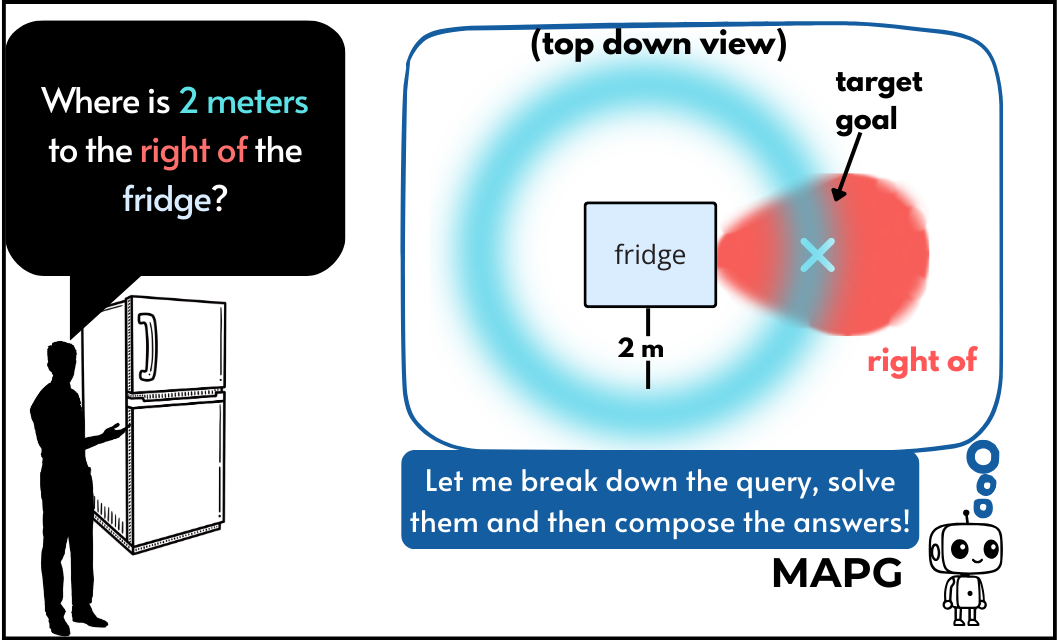
\includegraphics[width=1\linewidth]{figures/introfigure-rework.png}
    \caption{When a human specifies an open world metric-semantic query, referring to a location in the world, MAPG decomposes the query into subparts as learned probability distributions and composes them for grounding.
    }
    \label{fig:overview}
\end{figure}
Grounding these metric-semantic queries in a map requires jointly reasoning over referent semantics, spatial predicates, and metric scale, where the intended goal is a continuous region anchored to a grounded object pose.
%\ngnote{make this para tighter. I took a pass but it might have some facts missing. Also there is an argument to be made about single models needing more data when compared to using existing models compositionally.} \opnote{yes, read and use language from here: https://arxiv.org/abs/2402.01103v3.}

Instruction following is a central subfield of grounded language learning in robotics \cite{tellexlanguagesurvey}. Most existing systems ground language to actions or goals, which can be objects in a scene \cite{dai2024thinkactaskopenworld}. %\tn{https://arxiv.org/pdf/2310.07968, https://openreview.net/pdf?id=nNsZxc2cmO}. 
Several grounded language systems emphasized structured decomposition and probabilistic inference to connect linguistic constituents to world entities~\cite{tellex2011symbolgrounding}  while modern navigation and embodied question answering (QA) systems increasingly rely on large vision-language models (VLMs) and large language models (LLMs) to reason over observations and internal scene representations such as $3$D semantic scene graphs \cite{graphEQA, rana2023sayplan}. %\ngnote{whole line of work from cynthia matuszek and hadas kresgazit going from language to goals as well}
These approaches treat goal grounding as a single-step decision: given the current observation (and sometimes an internal map), the model is prompted to output either a discrete action or a single target hypothesis \cite{vsiBench,frameOfReferenceAmbiguity}.  However, such designs can be fragile for metric-semantic instructions whose correctness depends on precise geometry and a consistent frame of reference while navigating to discover the goal.
Furthermore, language grounding is bidirectional: the agent must convert egocentric observations into allocentric positions on the map, then convert an allocentric goal back into egocentric coordinates for execution, which compounds errors from each step.
% Since the system typically commits early to one target, recovery often reduces to heuristic retries rather than principled re-grounding in a persistent $3$D representation \cite{vsiBench,frameOfReferenceAmbiguity}.
% In embodied navigation, an agent typically receives egocentric sensory inputs over time and builds an allocentric spatial memory that supports planning.
% $3$D scene graphs are one such representation of the environment: they store object nodes with estimated poses and geometry, and support querying the environment in an object-centric and spatially structured way and it helps connect language to persistent world state, but metric-semantic goal grounding remains challenging under viewpoint changes, partial observability, and ambiguous frames of reference \cite{vsiBench,frameOfReferenceAmbiguity}.

% Existing embodied systems still struggle with metric-semantic goal grounding: general-purpose LLMs are unreliable for fine-grained metric spatial reasoning, and even scene-graph-based approaches often reduce goals to discrete targets rather than continuous spatial intent \cite{graphEQA}. These trends suggest a missing piece in the reasoning stack: a representation that is grounded for control, flexible to represent and update uncertainty, and compositional to support complex spatial instructions. We address this gap with Multi-Agent Probabilistic Grounding (MAPG), an agentic framework that produces planner-ready goal distributions for metric-semantic spatial instructions and add a probabilistic goal interface between foundation-model grounding signals and navigation affordances, representing the intended goal as a robust continuous distribution \(P(x)\) over $3$D space rather than as a single discrete target.

We propose MAPG (Multi-Agent Probabilistic Grounding), an agentic framework that queries different VLM Agents to produce probabilistic distributions and composes them into the goal. Given an instruction, MAPG decomposes it into structured clauses, resolves referents against an online $3$D scene graph and the current egocentric view, and instantiates analytic kernels for semantic, metric, and spatial constraints.
These kernels are then composed to produce a final goal density that better represents the spatial intention, which a planner can then query to generate executable waypoints.
Fig. \ref{fig:overview} shows an example of this approach.
%\opnote{also claim potentially better performance due to the fact that we can use expert models that are better at different aspects such as spatial reasoning.}
% \tn{cut: We instantiate this approach in a multi-agent architecture, that builds on the strengths of online $3$D scene graphs, composition and agentic frameworks.
% MAPG separates referent grounding from spatial inference: a Grounding Agent matches linguistic anchors (e.g., \emph{fridge}) to object instances in the scene graph using egocentric evidence, and a Spatial Agent outputs the parameters of the continuous probability field anchored at the resolved referent, which is then analytically composed into the final goal distribution.
% The planner then queries this goal distribution to propose candidate waypoints and selects a navigation action.}
%\opnote{talk more about the different agents you instantiate in the scene, what they return at a high level (parameters of a distribution) and how you compose them at a high level.}\ljnote{subsection 1 in method, could be moved here.} \tn{I only want a sentence, something like: We pre-specify the shape of the kernels and use different models to predict the kernel parameters based on...} 
% We evaluate this framework in Habitat simulation using HM$3$D scenes \cite{ramakrishnan2021habitatmatterport$3$Ddatasethm$3$D}, with a curated set of annotated metric-spatial queries that target object-to-world relationships in cluttered indoor environments. 
% We release this dataset and evaluation protocol to support reproducible comparison for metric-semantic goal grounding, and report results against VLM-based baselines and scene-graph-driven planners. 

Our main contributions are as follows: %\opnote{be more emphatic- and not dry in your contributions}:
\begin{itemize}
    \item \textbf{A multi-agent probabilistic $3$D spatial reasoning framework for goal grounding} that couples online $3$D scene graphs with analytically defined continuous spatial kernels to produce planner-ready goal distributions for metric-semantic instructions.
    \item \textbf{A first-of-its-kind HM$3$D~\cite{ramakrishnan2021habitatmatterport3ddatasethm3d} goal grounding benchmark for metric-semantic queries}, including an open-source dataset and evaluation protocol spanning $41$ unique indoor scenes and $98$ annotated metric-semantic queries designed for object-to-world goal grounding in realistic indoor layouts.
    \item \textbf{Empirical findings and ablations}: In a completed $98$-query end-to-end evaluation, MAPG succeeds on $79$ queries ($80.6\%$) and finds the anchor on $80$ ($81.6\%$). We additionally report predicate-level and target-distance breakdowns and provide a failure taxonomy for reproducible comparison.
\end{itemize}
Our webpage includes videos, benchmark examples, and extensive results: \opnote{website is not working} \href{https://sites.google.com/view/mapg-web/home}{sites.google.com/view/mapg-web/home}.
% full-width figure right after contributions
% \clearpage % optional: forces the page break here (use ONLY if you want to guarantee the break)
\begin{figure*}[t]
    \centering
    \vspace{1mm}
    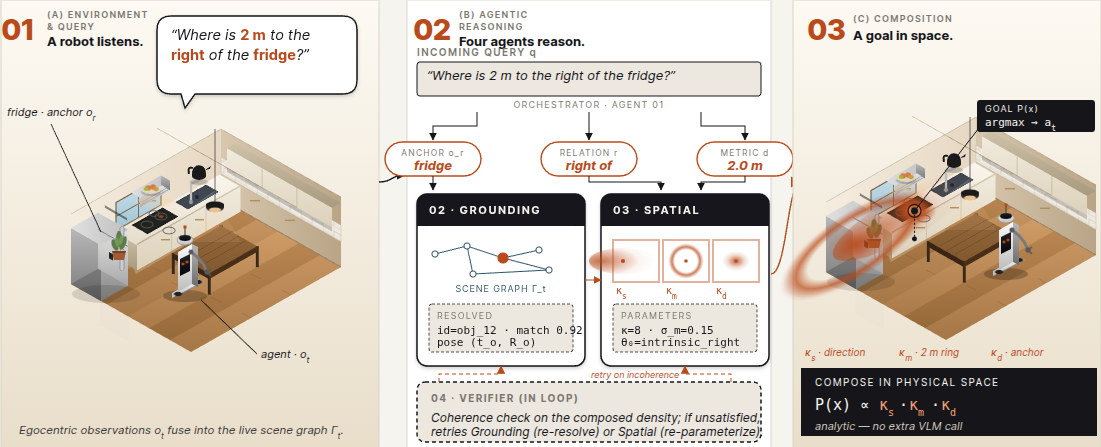
\includegraphics[width=0.99\linewidth]{figures/figure_2_new.png}
    \caption{\textbf{MAPG overview.}
    (a)~The robot observes a $3$D environment and receives a natural-language spatial query $q$.
    (b)~\emph{Agentic spatial reasoning layer}: the Orchestrator decomposes $q$ into anchor, relation, and metric tokens $\langle o_r, r, d\rangle$; the Grounding Agent resolves $o_r$ against the $3$D scene graph $\Gamma_t$ using multi-view evidence; the Spatial Agent emits parameters for the directional, metric, and anchor-density kernels. The Verifier closes a retry loop on incoherent compositions.
    (c)~\emph{Composition layer}: MAPG composes the analytic kernels in physical space to produce a continuous target-location PDF $P(x)$, planner-ready as a navigation or object-selection goal. \opnote{too much empty space}
    % \opnote{You don't talk about the logical agent in your methods section. The methods section and these diagrams need to present a consistent picture, and that is very important.}
    }
    \label{fig:method-overview}
\end{figure*}
